\documentclass[a4paper,11pt]{report}


%%%%%%%%%%%%%%%%%%%%%%%%%%%%
% University of Sussex thesis template
%%%%%%%%%%%%%%%%%%%%%%%%%%%%
% Modification History
%
% Based on usthesis.cls by Jonathon Read
% http://www.cogs.susx.ac.uk/users/jlr24/latex.html
% Modified by Anthony Smith, Feb 2007
% Incorporated into single thesis.tex file, Anthony Smith, 30 June 2008
% Minor alterations to page numbering, AJS, 25 July 2008
% New alternative hyperref options for print version, AJS, 11 Sep 2008
% "DRAFT" on header, AJS, 12 Sep 2008
%%%%%%%%%%%%%%%%%%%%%%%%%%%%


%%%%%%%%%%%%%%%%%%%%%%%%%%%%
% LINE SPACING 
\newcommand{\linespacing}{1.5}
\renewcommand{\baselinestretch}{\linespacing}
%%%%%%%%%%%%%%%%%%%%%%%%%%%%

%%%%%%%%%%%%%%%%%%%%%%%%%%%%
% CUSTOM COMMAND
\newcommand\ddfrac[2]{\frac{\displaystyle #1}{\displaystyle #2}}
%%%%%%%%%%%%%%%%%%%%%%%%%%%%

%%%%%%%%%%%%%%%%%%%%%%%%%%%%
% BIBLIOGRAPHY STYLE
\usepackage{natbib}
% \bibliographystyle{plain} for [1], [2] etc.
\bibliographystyle{apalike}
%%%%%%%%%%%%%%%%%%%%%%%%%%%%


%%%%%%%%%%%%%%%%%%%%%%%%%%%%
% OTHER FORMATTING/LAYOUT DECLARATIONS
% Graphics
\usepackage{graphicx,color}
\usepackage{epstopdf}
\usepackage[british]{babel}
% The left-hand-side should be 40mm.  The top and bottom margins should be
% 25mm deep.  The right hand margin should be 20mm.
\usepackage[a4paper,top=2.5cm,bottom=2.5cm,left=4cm,right=2cm,headsep=10pt]{geometry}
\flushbottom
% Pages should be numbered consecutively thorugh the main text.  Page numbers
% should be located centrally at the top of the page.
\usepackage{fancyhdr}
\fancypagestyle{plain}{
	\fancyhf{}
	% Add "DRAFT: <today's date>" to header (comment out the following to remove)
	\lhead{\textit{DRAFT: \today}}
	%
	\chead{\thepage}
	\renewcommand{\headrulewidth}{0pt}
}
\pagestyle{plain}
%%%%%%%%%%%%%%%%%%%%%%%%%%%%


%%%%%%%%%%%%%%%%%%%%%%%%%%%%
% ANY OTHER DECLARATIONS HERE:

%%%%%%%%%%%%%%%%%%%%%%%%%%%%


%%%%%%%%%%%%%%%%%%%%%%%%%%%%
% HYPERREF
\usepackage[colorlinks,pagebackref,pdfusetitle,urlcolor=blue,citecolor=blue,linkcolor=blue,bookmarksnumbered,plainpages=false]{hyperref}
\usepackage{amssymb}
\usepackage{amsmath}
% For print version, use this instead:
%\usepackage[pdfusetitle,bookmarksnumbered,plainpages=false]{hyperref}
%\usepackage{backref}
%\renewcommand{\backrefpagesname}{Cited on}
%%%%%%%%%%%%%%%%%%%%%%%%%%%%


%%%%%%%%%%%%%%%%%%%%%%%%%%%%
% BEGIN DOCUMENT
\begin{document}
%%%%%%%%%%%%%%%%%%%%%%%%%%%%


%%%%%%%%%%%%%%%%%%%%%%%%%%%%
% PREAMBLE: roman page numbering i, ii, iii, ...
\pagenumbering{roman}
%%%%%%%%%%%%%%%%%%%%%%%%%%%%


%%%%%%%%%%%%%%%%%%%%%%%%%%%%
%% TITLE PAGE: The title page should give the following information:
%%	(i) the full title of the thesis and the sub-title if any;
%%	(ii) the full name of the author;
%%	(iii) the qualification aimed for;
%%	(iv) the name of the University of Sussex;
%%	(v) the month and year of submission.
\thispagestyle{empty}
\begin{flushright}

\includegraphics[width=6cm]{uslogo}
\end{flushright}	
\vskip40mm
\begin{center}
% TITLE
\huge\textbf{My Theory of Everything}
\vskip2mm
% SUBTITLE (optional)
\LARGE\textit{How it all works}
\vskip5mm
% AUTHOR
\Large\textbf{Joe Bloggs}
\normalsize
\end{center}
\vfill
\begin{flushleft}
\large
% QUALIFICATION
Submitted for the degree of Doctor of Philosophy \\
University of Sussex	\\
% DATE OF SUBMISSION
September 2008
\end{flushleft}		
%%%%%%%%%%%%%%%%%%%%%%%%%%%%


%%%%%%%%%%%%%%%%%%%%%%%%%%%%
% DECLARATIONS
\chapter*{Declaration}
I hereby declare that this thesis has not been and will not be
submitted in whole or in part to another University for the award of
any other degree.
	
% ADDITIONAL DECLARATIONS HERE (IF ANY)

\vskip5mm
Signature:
\vskip20mm
% AUTHOR
Joe Bloggs
%%%%%%%%%%%%%%%%%%%%%%%%%%%%


%%%%%%%%%%%%%%%%%%%%%%%%%%%%
% SUMMARY PAGE
\thispagestyle{empty}
\newpage
\null\vskip10mm
\begin{center}
\large
\underline{UNIVERSITY OF SUSSEX}
\vskip20mm
% AUTHOR, QUALIFICATION
\textsc{Joe Bloggs, Doctor of Philosophy}
\vskip20mm
% TITLE
\underline{\textsc{My Theory of Everything}}
\vskip0mm
% SUBTITLE (optional)
\underline{\textsc{How it all works}}
\vskip20mm
\underline{\textsc{Summary}}
\vskip2mm
\end{center}
% Change line spacing
\renewcommand{\baselinestretch}{1.0}
\small\normalsize
% SUMMARY HERE (300 word limit for most subjects):

%%%%%%%%%%%%%%%%%%%%%%%%%%%%


%%%%%%%%%%%%%%%%%%%%%%%%%%%%
% ACKNOWLEDGEMENTS
\chapter*{Acknowledgements}
\renewcommand{\baselinestretch}{\linespacing}
\small\normalsize
% ACKNOWLEDGEMENTS HERE:

%%%%%%%%%%%%%%%%%%%%%%%%%%%%


%%%%%%%%%%%%%%%%%%%%%%%%%%%%
% TABLE OF CONTENTS, LISTS OF TABLES & FIGURES
\newpage
\pdfbookmark[0]{Contents}{contents_bookmark}
\tableofcontents
\listoftables
\phantomsection
\addcontentsline{toc}{chapter}{List of Tables}
\listoffigures
\phantomsection
\addcontentsline{toc}{chapter}{List of Figures}
%%%%%%%%%%%%%%%%%%%%%%%%%%%%


%%%%%%%%%%%%%%%%%%%%%%%%%%%%
% MAIN THESIS TEXT: arabic page numbering 1, 2, 3, ...
\newpage
\pagenumbering{arabic}
%%%%%%%%%%%%%%%%%%%%%%%%%%%%


%-----------------------------------------------------
% Chapter: Introduction
%-----------------------------------------------------

% NB Good idea to put each chapter in a separate file.
% If you put the following in a file called "thesis_introduction.tex"
% then you can include it with the following:

\chapter{Introduction}
\label{chap:intro}

% This is the introduction to the thesis.\footnote{And this is a
% footnote.}  The conclusion is in Chapter on page.
\section{Motivation} 
    Word embedding is a method for word representation mainly used in
    natural language processing domain. However, text data represented
    differently in machine unlike images and sounds data. Generally
    image is represented as two-dimensional to four-dimensional (given
    channels and alpha value) matrix with finite number of cell
    elements containing numerical value to represent color intensity
    on each location \citep{imageprocessing2018tyagi}. For example RGB
    image represented with 3-dimensional matrix. Each dimension
    represents the intensity of red color, green color, and blue color
    respectively in form of two-dimensional matrix. On the other hand,
    sound is represented as one-dimensional signal or stack of those
    signals (given several channels, it becomes two-dimensional)
    representing air pressure in the ear canal (for instance one
    channel for the left ear and one for the other)
    \citep{sound1995rocchesso}. Both images and sounds can be easily
    represented as mathematical models either using analog or digital
    signals but not with text data \citep{wordembedding2017yang}.
    Hence word embedding was introduced to give ability in
    representing text as a mathematical model namely a vector.
    
    Text data consists of sequence of characters that is represented
    by codes that is standardized, for example ASCII. In ASCII each
    character is represented by a number from $0$ to $127$ that later
    on extended until $255$. Combinations of these number then
    translated by computer to represent a character. Originally, in
    natural language processing text data can only be modeled using
    one-hot vector. This vector is a one-dimensional vector that has
    $d$-dimension, given \textit{d} words that are known or used. Each
    word is represented by one dimension and depends on the used word
    entries in the sentence, the correspondent dimension's value is
    $1$ and the rest is $0$ hence the name one-hot vector. The one-hot
    vector then stacked with another one-hot vectors to represent
    order of use in a sentence. Similar representation is also used to
    represent characters. The problem with one-hot vector is that it
    does not have any information that infers connection between one
    to another. It only encodes that certain word is used in a certain
    sentence in a certain sequence. Instead of sparse representation
    for each word, dense vector representations that maps semantic and
    syntactic information between words given one-hot vectors in a
    Euclidean space is introduced \citep{wordembedding2017yang,
    Distributed2013mikolov}. Hopefully, this positional information
    can be used to infer interconnection between words, whether its
    similarities or usage of the word in a sentence
    \citep{distributional1954harris}. To obtain word embeddings, a
    model is created to extract features of a word from a corpus and
    map its location in Euclidean space based on the features found
    \citep{Distributed2013mikolov, polyglot2013alrfou,
    dict2vect2017tissier}. These word embeddings then can be used to
    do many downstream tasks, such as POS-tagging, named entity
    recognition (NER), and sentiment analysis \citep{finding2015ling,
    neural2016lample}. 

    In general, large corpus with many words and examples of word
    usage is preferred because the size of the vocabularies will be
    higher and more words connection can be inferred from the corpus
    \citep{size2018kutuzov}. On top of that, multiple use of a
    vocabulary might also be used as a training data as an examples of
    cases of vocabulary usage in a sentence. However, it is not
    possible to have enough corpus since the language itself is
    creative and changing overtime \citep{forrester2008abrief,
    speech2009Jurafsky:2009:SLP:1214993}. Furthermore, there are cases
    of typographical error, especially on social media platform where
    anybody willingly write text over these platforms
    \citep{Liu2010SentimentAA} and some of these words may not be
    present in the corpus hence not included in the vocabulary even
    though there is another word that has the exact similar meaning to
    those words thus it should more or less has close distance to the
    standard or original word \citep{mapping2012eisenstein}. In
    addition with the increasing number of smartphones which uses
    touch screen, increase of number in typographical error is to be
    expected \citep{ghosh2017correction}. All these non-existent words
    in the corpus because of inability to collect such corpus or
    simply because of emergence of new slang or typographical error
    making the embedding of such word is unknown and it is called as
    \textit{out-of-vocabulary} (OOV) words. One may use simple
    approach by assigning unique random embedding for every OOV or by
    replacing OOV with an unknown \textit{\textless UNK\textgreater}
    token with randomly initialized embedding
    \citep{predicting2019garneau}, that later hoped to be generalized
    in training. Despite the fact that it can be used for OOV, further
    improvement on downstream tasks should be able to be achieved by
    using machine learning method to infer OOV embeddings.

    To infer OOV embeddings, the proposed model will be built over
    quasi-generative perspective. Only knowing the vocabularies and
    its embedding, the embedding for OOV words will be generated by
    the model. Previous \textit{state-of-the-art} used LSTM to infer
    OOV embeddings called \textsc{Mimick} \citep{mimicking2017Pinter}.
    For this model to infer OOV embedding, character embedding was
    first randomly initialized with a set of characters as its
    vocabulary. The character embedding then used to transform
    sequence of characters in a word into sequence of embedding. The
    sequence of the character embeddings then forwarded into
    bidirectional Long-Short Term Memory (bi-LSTM) then to fully
    connected layer. In language model, bi-LSTM generally works by
    separating sub-word by remembering and forgetting previous
    sequence from both end. How LSTM works in connection to this
    problem will be further explained in chapter \ref{chap:method}.
    The last hidden state of the bi-LSTM then will be used to infer
    its embedding. By architecture of LSTM, the gates inside the
    hidden neuron might drop previous information. Hence a problem
    might arise when there are more than two important sub-words and
    they are not in sequence, meaning that there exist at least one
    character between two sub-words considered important, hence the
    information is incomplete since the previous information will be
    dampened by LSTM hidden neuron interiors if the next sequence of
    sub-words are considered more important. This problem will be
    explained further in chapter \ref{chap:method}. From the
    explanation above, proposal of a new method to handle OOV is
    created.

\section{Objectives}
    For OOV to be inferred, a model that are able to generate
    embedding for the correspondence word has to be created. In
    \textsc{Mimick}, the whole sequence is processed by a bi-LSTM. By
    the problem mentioned earlier, instead of taking the whole words
    as a sequence and considering its importance based on time and
    occurrence using bi-LSTM, n-grams will be used to pick which grams
    (set of sequence) that are considered to be important. In theory
    this method should gives better results in downstream tasks since
    the information fed is complete and only left for the model to
    pick which n-grams features are more important. The only problem
    is that for the model to pick which grams that should be included
    in the model is impossible to do since there are many word
    combinations making the model needs to accept huge number of
    inputs. Instead of handpicking the features of n-grams,
    convolutional neural network (CNN) can be used to learn the
    existed features and pick which features needs to be considered by
    using character embedding and treat the character sequence
    embedding as two-dimensional matrix. The features picked then will
    be processed to predict the word embedding for the input word
    using feedforward network.

\section{Contributions}
    \begin{enumerate}
        \item An improved OOV handling model for downstream task
        \item Evaluation on different settings for baseline model and
        the proposed model
    \end{enumerate}

\section{Thesis Structure}
    The remainder of this document is structured as follows. In the
    \nameref{chap:relatedwork} chapter, the previous works that are in
    relatives with research done in this documents are mentioned
    especially the baseline used in this research. In the following,
    \nameref{chap:preliminaries} chapter, base theories for
    feedforward neural network, recurrent neural network, and n-grams
    that are considered to be needed are explained in details here. On
    top of that, the problem of the previous \textit{state-of-the-art}
    will be explained in depth here. In the \nameref{chap:method}
    chapter, the method of solution proposed to the problem and the
    testing method for analyzing the results are explained. In the
    \nameref{chap:implementation} chapter, the method of solution
    proposed to the problem are described in technical way to show how
    it is implemented and tested. In the \nameref{chap:results}
    chapter, the results are shown and discussed with the relation
    with the previous \textit{state-of-the-art}. Lastly,
    \nameref{chap:conc} chapter talks about the conclusion that are
    able to be pulled from this research.
\chapter{Related Work}
\label{chap:relatedwork}

% This is the introduction to the thesis.\footnote{And this is a
% footnote.}  The conclusion is in Chapter on page
Polyglot is one of word embeddings that is focused on multilingual
application \citep{polyglot2013alrfou}. A total of one hundred and
seventeen languages word embeddings were generated to give
availability of different language models to be trained. Previously,
specific language features were hand crafted by experts of specific
language \citep{polyglot2013alrfou}. This makes applying a language
model that are trained with commonly available language features
harder, hence the creation of Polyglot word embedding
\citep{polyglot2013alrfou}. This embedding was trained using Wikipedia
article and has no OOV handling if there exist a word that is not used
in Wikipedia. This pre-trained embedding was also used in the baseline
model \textsc{Mimick} for generating OOV embedding in many languages.

Word2vec is another word embedding that was trained using skip-gram
model \citep{efficient2013mikolov}. The available language choice for
this pre-trained embedding is English. A word $w(t)$ used as an input
and its context word, for example context word with windows of 4 are
$w(t-2), w(t-1), w(t+1),$ and $w(t+2)$ are used as the target. The model
tried to project the input $w(t)$ to the output to predict the context
words \citep{efficient2013mikolov}. Similar with Polyglot, this model
is highly dependent on the corpus completeness. The more examples and
vocabularies a corpus has, the better the representation of the
embeddings will be since more information will be able to be retrieved.
Word2vec model has no OOV handling either, meaning either random
vector or unknown ``\textit{\textless UNK\textgreater}'' embedding
will be used for it.

Dict2vec is yet another embedding that was trained by looking up
definitions of words from Cambridge dictionary
\citep{tissier2017dict2vec}. This embedding was created because the
previous method is trained with an unsupervised manner, which means that
there is no supervision between pairs of words. There might exists
a pair of words that are highly related but do not appear enough
inside a corpus which makes it harder for the model to find a connection
\citep{tissier2017dict2vec}. Thus, this model was trained by creating
sets of strong and weak pairs of words, then move both pairs closer
and further respectively based on the pairs. The model was evaluated by
using several word similarity tasks to show improvements over vanilla
implementation of word2vec and fasttext \citep{tissier2017dict2vec}.
Similar with previous word embedding, Dict2vec also has no OOV
handling method and since the vocabularies were only inferred from
Cambridge dictionary, there is no typographical error.

As aforementioned above, those word embedding has no way of handling
OOV words other than by assigning some unknown token
``\textit{\textless UNK\textgreater}'' or by letting the downstream
tasks model to train from the randomly generated embeddings each time
an OOV emerges. This case fueled \textsc{Mimick}, an OOV handling
model to be created \citep{mimicking2017Pinter}. This model was able
to tackle this problem successfully by using bi-directional long-short
term memory (bi-LSTM) to process embedding of characters of an OOV
word to produce the word embeddings. The OOV embedding generation
process was taken from quasi-generative perspective, which means that
the original embedding was assumed to has some form that could
generate the embeddings \citep{mimicking2017Pinter}. By doing so, the
OOV embeddings were able to be predicted without the needs of knowing
lexicon or model used for creating the word embedding. To prove that
such OOV handling model could perform better than randomly generated
embeddings or unique embedding for unknown token ``\textit{\textless
UNK\textgreater}'', several downstream tasks were used to evaluate the
model, such as Part-of-Speech-Tagging (POS-tagging) and word
similarity task that will be explained further below.

Part-of-Speech-Tagging (POS-tagging) is a process of determining
grammatical category called a \textit{tag} of a given word in a certain
sentence. In English, there are words that has ambiguous grammatical
category, such as word ``tag'' can either be noun or verb depending on
the usage of it \citep{apractical1992cutting}. To tackle this problem,
many researchers proposed to use of mathematical models or statistical
models namely hidden Markov model \citep{apractical1992cutting},
n-grams \citep{tnt2000Brants}, and neural network model
\citep{finding2015ling}. In this research, the neural network model
would be implemented to serve as the downstream task. This model was a
bi-LSTM that took sequence of word embeddings to represent a sentence
or parts of sentence then each word embedding were categorized for its
tag based on the usage in that sentence.

In spite of the performance of \textsc{Mimick}, there are evidence
of CNN that is used for sequence modeling can outperform LSTM and
RNN architecture \citep{empirical2018shaujie}. Moreover, CNN converges
faster than LSTM, RNN, and GRU based on the number of iteration
despite of the sequence length \citep{empirical2018shaujie}. The model
called temporal convolution network (TCN) is basically a multilayer
CNN with different dilation to factor the collection of input
dimension for each layer. The model was evaluated by using several
sequence modelling tasks.

For training an OOV model, some kind of feature extraction method
needs to be used. One of feature extraction method called n-grams is
often used to capture word features. N-grams can be applied in both
character grams in a word or word grams in a sentence. With character
embedding and convolution neural network (CNN), n-grams can be
calculated by convoluting sets of characters embedding with the kernel
size of $n \times d$ for $n$ is the number of grams and $d$ is the
dimension of the embeddings. This CNN n-grams then can be used to
create a neural language model \citep{character2015kim}.

\cite{character2015kim} created a language model for several
languages. This model used character n-grams by using character
embeddings and processed with CNN like an image. The results from
these process then passed through a highway network. A highway network
controls whether the information from the input would also be carried
to the next process or to be changed with original embedding or ASCII
code. The output of the highway network then passed through LSTM to
predict the next word. In those research, the results of the model for
OOV nearest neighbor trained with or without highway network were
compared. The results was that the one trained without highway network
has closer distance to a word that has smallest edits while the one
that trained with the highway network has closer distance to a word
with similar orthographic \citep{character2015kim}.

\cite{batchnorm:DBLP:journals/corr/IoffeS15} proposed a model to
compensate slower training time caused by internal covariate shift.
This phenomenon happened because the distribution of values changes
between layers in neural network, making training model that saturates
to a nonlinearity activation function harder
\citep{batchnorm:DBLP:journals/corr/IoffeS15}. By using a method
called Batch Normalization, each layer's inputs were normalized to
match distribution of certain mean and variance. As a result, larger
learning rates can be used and smaller training epoch was needed to
achieve a certain error values compared to the one without Batch
Normalization \citep{batchnorm:DBLP:journals/corr/IoffeS15}.
\chapter{Method}
\label{chap:method}

% This is the introduction to the thesis.\footnote{And this is a
% footnote.}  The conclusion is in Chapter on page
\section{Out-of-Vocabulary Model}
    \subsection{Sequence Feature Extraction}
        OOV problem is handled from quasi-generative perspective as
        aforementioned in chapter \ref{chap:intro} by using neural
        language model under assumption that there is a form that
        could generate embedding for the original embedding. Hence
        that, the original embedding is used for training the model to
        generate the embedding. In chapter \ref{chap:intro}, reasons
        why lstm could perform worse is because the hidden states is
        controlled by cell gates making the information that is
        carried on is the most recent after the cell gates decided to
        forget inputs at certain time $t$. 

        \begin{align}
            \label{eq:lstm:f_t}
            f_t &= \sigma(W_f \cdot [h_{t-1}, x_t] + b_f) \\
            \label{eq:lstm:i_t}    
            i_t &= \sigma(W_i \cdot [h_{t-1}, x_t] + b_i) \\
            \label{eq:lstm:Cc_t}
            \tilde{C}_t &= tanh(W_C \cdot [h_{t-1}, x_t] + b_C) \\
            \label{eq:lstm:C_t}
            C_t &= f_t \times C_{t-1} + i_t \times \tilde{C}_t \\
            \label{eq:lstm:o_t}
            o_t &= \sigma(W_o \cdot [h_{t-1}, x_t] + b_o) \\
            \label{eq:lstm:h_t}
            h_t &= o_t \times tanh(C_t)
        \end{align}

        Formally, when $C_t = 0$ from equation \ref{eq:lstm:C_t},
        hidden state from equation \ref{eq:lstm:h_t} will be reset to
        $0$ rendering hidden states prior to time $t$ gone. This
        problem can be solved by using bi-lstm, since bi-lstm process
        sequence in forward and reverse order making both early and
        later sequence held by the last hidden state for each forward
        lstm and reverse lstm respectively. Another problem might
        arise when we need to divide sequence into more than three
        subsequence as shown on figure \ref{fig:subsequence}. Hence
        another approach is needed since intermediate subsequence
        might get deleted or carried along with the later sequence
        even with bi-lstm.

        \begin{figure}
            \begin{align*}
                &un \vert recogniz \vert able \\
                &inter \vert national \vert ities \\
                &oto \vert rhino \vert laryngolog \vert ical \\
                &hepatico \vert chol \vert angio \vert gastro \vert stomy
            \end{align*}
            \caption{Word examples with three or more subsequences}
            \label{fig:subsequence}
        \end{figure}

        We can find many examples especially from more technical areas
        as shown on figure \ref{fig:subsequence}. Since on
        \textsc{Mimick} \cite{mimicking2017Pinter} implementation only
        the last hidden state is used for inferencing word embedding,
        another approach is proposed.

        \begin{figure}
            \begin{align*}
                unrecognizable : &unre \vert nrec \vert reco \vert ecog \vert cogn \vert ogni \vert gniz \vert niza \vert izab \vert zabl \vert able\\
                internationalities : &inte \vert nter \vert tern \vert erna \vert rnat \vert nati \vert atio \vert tion \vert iona \vert onal \vert \\
                &nali \vert alit \vert liti \vert itie \vert ties\\
                otorhinolaryngological : &otor \vert torh \vert orhi \vert rhin \vert hino \vert inol \vert nola \vert olar \vert lary \vert \\
                &aryn \vert ryng \vert yngo \vert ngol \vert golo \vert olog \vert logi \vert ogic \vert gica \vert ical\\
                hepaticocholangiogastrostomy : &hepa \vert epat \vert pati \vert atic \vert tico \vert icoc \vert coch \vert ocho \vert chol \vert hola \vert olan \vert\\
                &lang \vert angi \vert ngio \vert giog \vert ioga \vert ogas \vert gast \vert astr \vert stro \vert\\
                &tros \vert rost \vert osto \vert stom \vert tomy
            \end{align*}
            \caption{4-grams examples}
            \label{fig:4grams}
        \end{figure}

        For all subsequence to be processed, we need a method that
        accounts for all sequence yet still able to divides the whole
        sequence into subsequences. Consequently, n-grams is chosen
        because this method splits word into sequence of characters
        depends on the chosen window size as shown on figure
        \ref{fig:4grams}. Those sequences of characters then feed into
        learning algortihm. This idea is similar to how human tries to
        recognize an unseen word by reading subword that is
        understandable beforhand when no explanation or context were
        given. 

        This model then will be used to estimate OOV embeddings. In
        other words, given sets of vocabulary $\mathcal{V}$ with size
        $\vert\mathcal{V}\vert$ and pretrained embeddings
        $\mathcal{W}^{\vert\mathcal{V}\vert \times d}$ for each word
        $w_{i} \in \mathcal{V}$ that is represented as a vector $e_i$
        with $d$ dimension, the model is trained to map function
        $f:\mathcal{V} \rightarrow \mathbb{R}^d$ that minimizes $\vert
        f(w_i) - e_i
        \vert^{2}$. This approach is similar to \textsc{Mimick}
        \cite{mimicking2017Pinter} approach. The text input is
        represented as a sequence of character $[c_1, c_2, \dots,
        c_m]$ for $c_i \in \mathcal{C}$. Those sequence then
        transformed as sequence of vectors $g_i$ with $b$ dimension by
        using character embeddings $\mathcal{G}^{\vert \mathcal{C}
        \vert \times b}$. For simplicity, sequence of $[g_1, g_2,
        \dots, g_m]$ will be called $[\hat{g}]$. $[\hat{g}]$ becomes
        2-dimensional matrix that has size of $m \times b$. In
        summary, given word $w$ will be transformed using function $h$
        into $[\hat{g}]$ as shown on equation \ref{eq:word2charemb}.

        \begin{equation}
            \label{eq:word2charemb}
            h: w \rightarrow [\hat{g}]
        \end{equation}

        To process $[\hat{g}]$ like an n-grams, CNN is used. CNN is
        basically a method to do convolution on matrix by using a
        kernel $k_i^{n \times b} \in K$. This operation is represented
        with $*$ symbol. To mimick n-grams, kernel with size of $n
        \times b$ is used, producing another vector $\hat{l}$ that
        represents the value of each grams, then non-linearity is
        applied to this vector by using ReLU activation function as
        shown in equation \ref{eq:relu}.

        \begin{equation}
            \label{eq:relu}
            f(x) = ReLU(x) = max(0,x)
        \end{equation}

        Several kernel is used to learn several features for producing
        embeddings. Each of these kernel will be responsible to find
        grams that are affecting the results, thus the vector
        $\hat{l_i}$ that are results of convolution $[\hat{g}] * k_i$
        will be maxpooled to produce one number. In details, from
        given sequence of character embedding $[\hat{g}]$, only gram
        that produces the highest value when convoluted by using
        kernel $k_i$ will be processed. Since, there are $\vert K
        \vert$ number of filter, $\vert K \vert$ number of grams will
        be considered to be important to the results. Furhtermore, by
        using several window sizes for n-grams (bigram, trigram,
        etc.), more features will be able to be learned.

    \subsection{Embedding Generation}
        After the features are able to be extracted, those features
        then concatenated and fed into fully connected layer with
        output size matching the pretrained embedding $\mathcal{W}$
        dimension $d$ with non-linear activation function matching the
        maximum and minimum bound of the pretrained embedding
        $\mathcal{W}$ resulting a new embedding vector $\tilde{e}$.

        The complete process from input word, feature extraction,
        until predicting embedding is shown on figure \ref{fig:model}.
        
        \begin{figure}
            \centering
            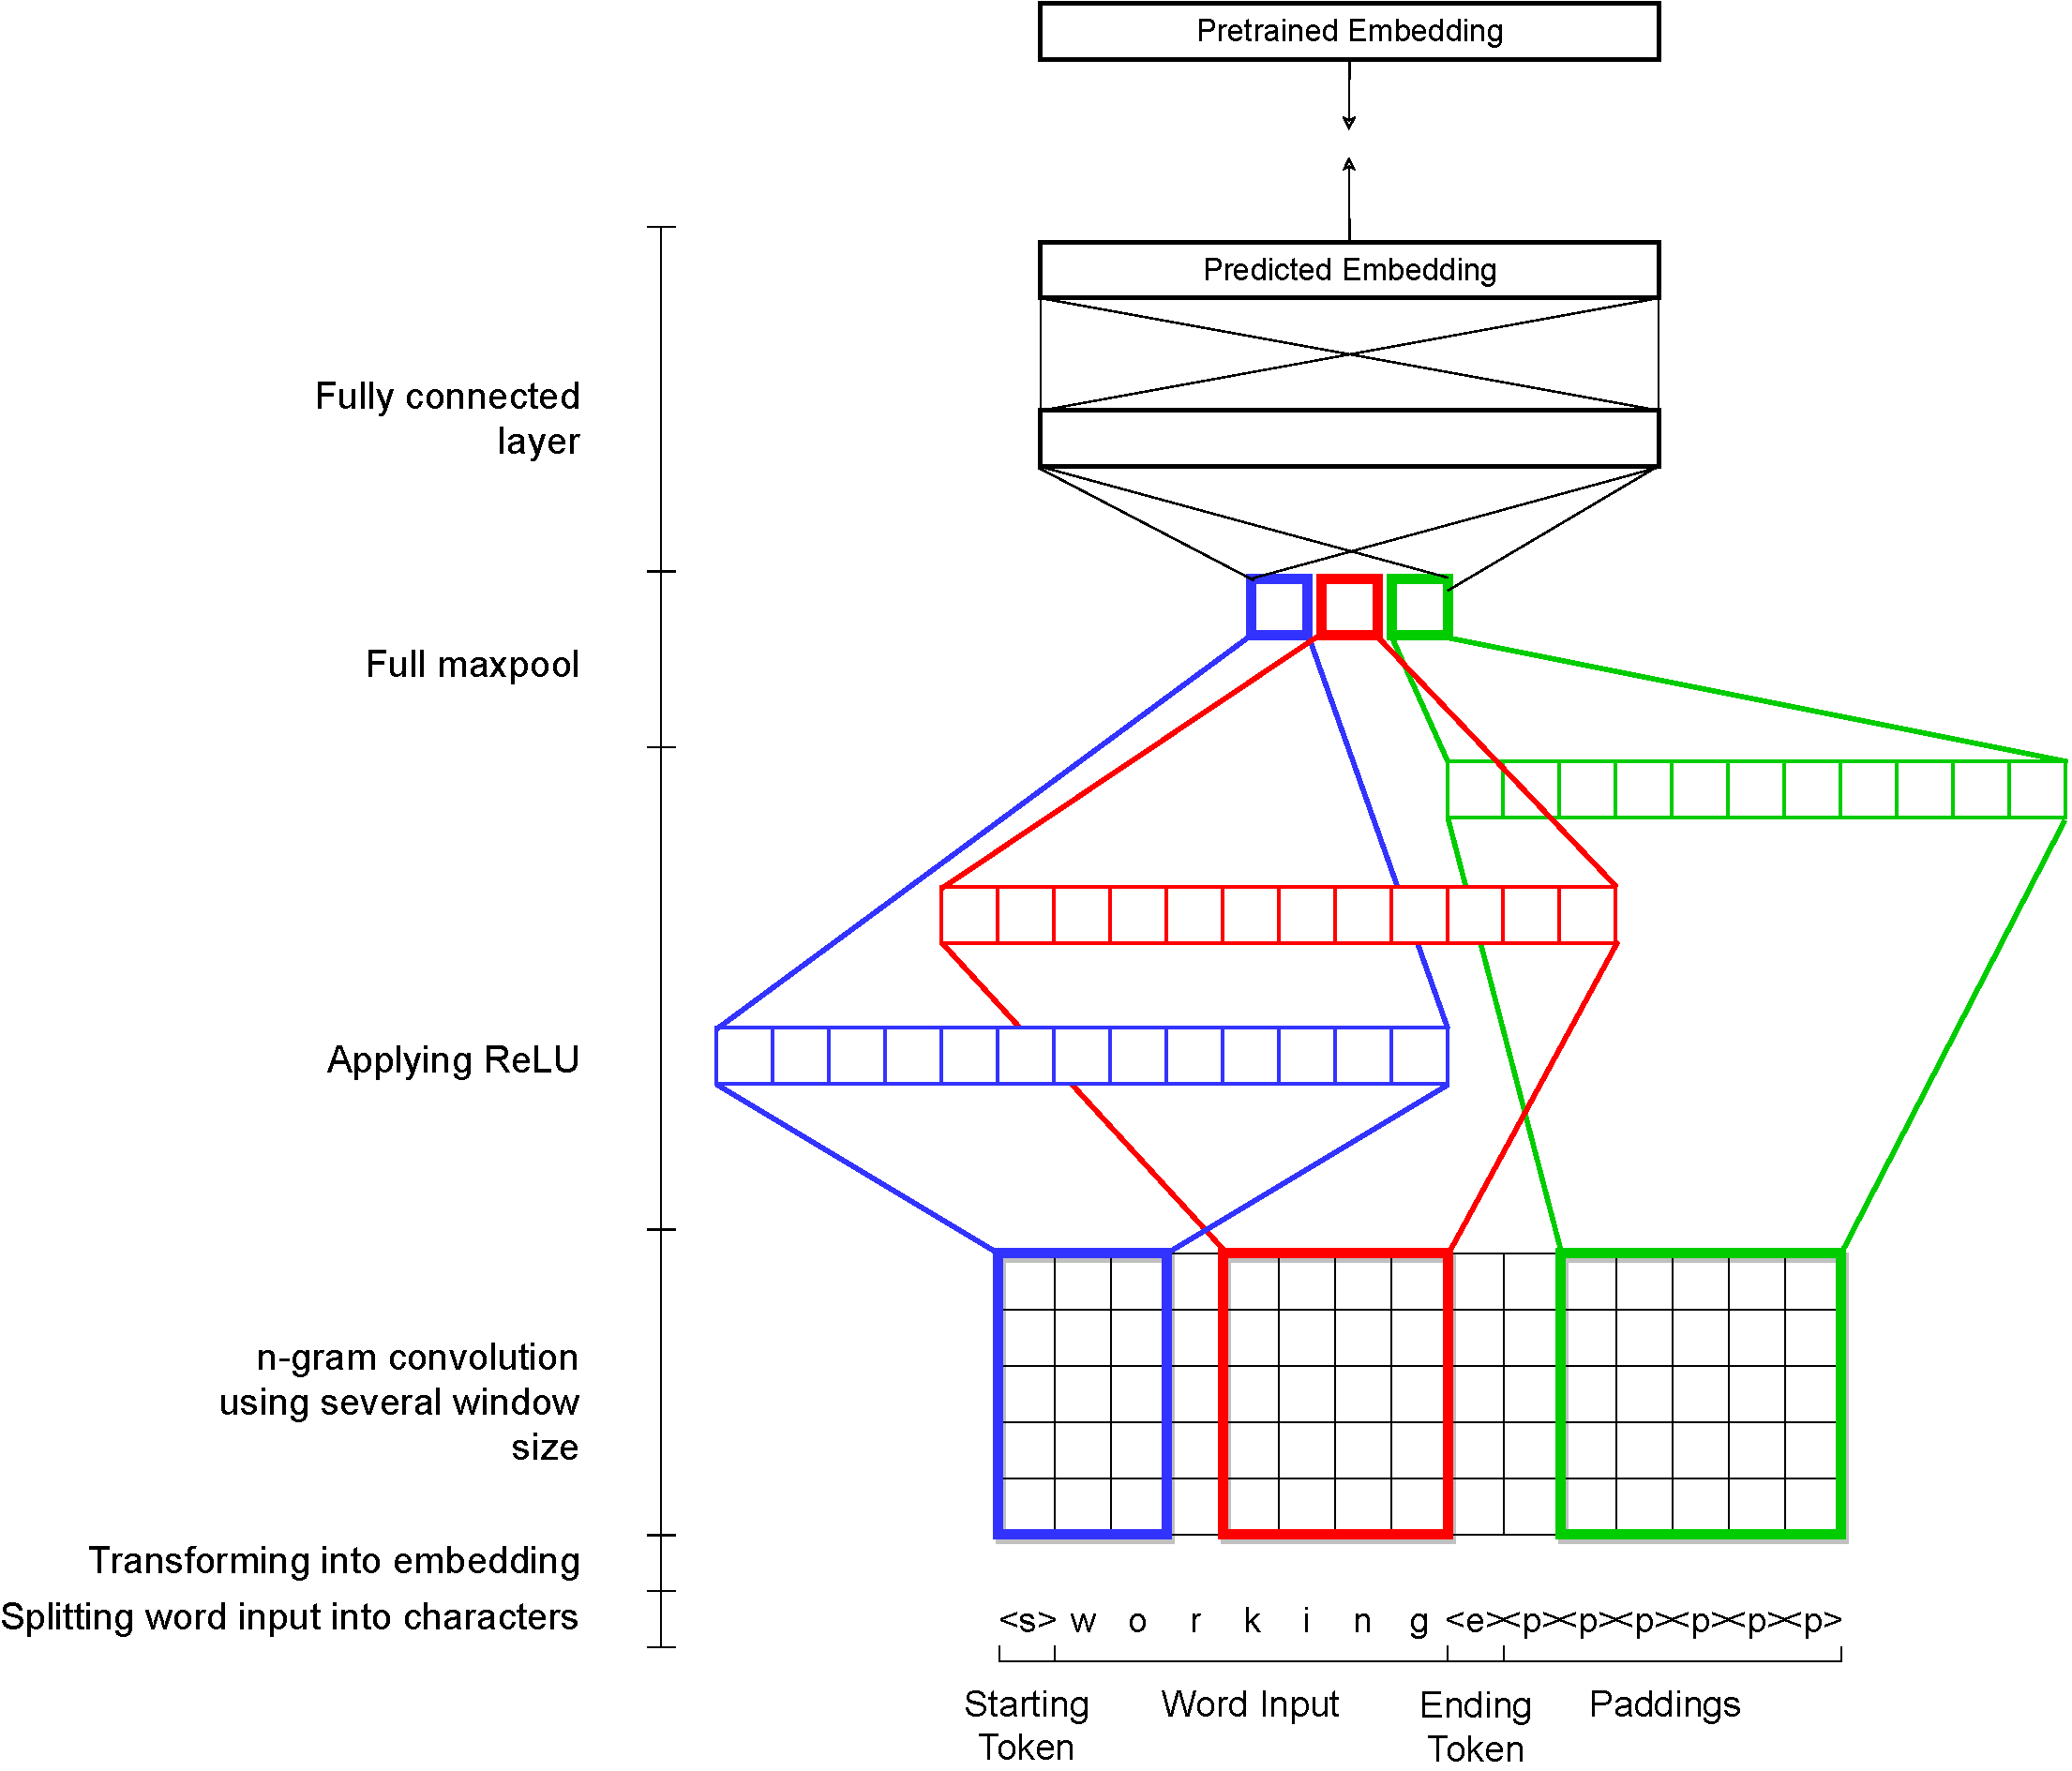
\includegraphics[width=.8\linewidth]{images/model.pdf}
            \caption{OOV Inferencing Model}
            \label{fig:model}
        \end{figure}

        On figure \ref{fig:model}, starting and ending token is added
        at the beginning and the end of the word respectfuly.
        Furthermore, padding token is added if the input word is
        shorter than the length of the input size of the model. The
        padding token is a zero vector $\vec{0}$ and $\vec{0} * k =
        \vec{0}$ for any $k$. This is to ensure that part of input
        that got padded does not goes through maxpool layer since only
        grams that has highest value can goes through the next layer
        and minimum value of ReLU is 0.

    \subsection{Error and Backpropagation}
        The output of the neural network $\tilde{e}$ then compared
        with the original embedding $e$ to learn new parameters for
        the neural network using mean squard error function as shown
        on \ref{eq:errorf}

        \begin{equation}
            \label{eq:errorf}
            Error = \frac{1}{2} \Vert e - \tilde{e} \Vert ^{2}
        \end{equation}

        The error then backpropagated to fine-tune the neural network
        parameters.
        
\section{Measuring Performance on Donwstream Tasks}
    In natural language modeling (NLP), there are several tasks that
    make used of word embedding. Hence that, the generated embeddings
    from the model can be evaluated by using those downstream tasks.
    The results then compared with the state-of-the-art OOV handling
    model \textsc{Mimick} \cite{mimicking2017Pinter}.
    
    \subsection{Part-of-Speech Tagging}
        Part-of-speech tagging or POStagging is a task of classifying
        words in sentence or corpus based on the grammatical usage of
        the word \{cite\}, for example: verb, noun, adverb, etc. Given
        sentence $S = \{w \in \mathcal{V} \vert ((w_1, t_1), (w_2,
        t_2), \dots, (w_n, t_n)\}$ with its POS-tag $t_i$, each word
        $w_i \in S$ is converted into sequence of character then each
        character is converted into character embedding $[\hat{g}]_i$
        using model represented in equation \ref{eq:word2charemb}.

        The sequence of character embeddings $[\hat{g}]_i$ then fed
        into bi-lstm with logsoftmax activation function at the output
        to get the POS-tag. To ease up computation time, adaptive
        logsoftmax is used \cite{grave2018efficientsoftmax}. Instead
        of calculating the whole classification, the frequent and
        infrequent classes are separated thus there are many chance
        that only frequent classes needs to be calculated. The
        complete process of postagging process is shown in figure
        \ref{fig:postag}.

        \begin{figure}
            \centering
            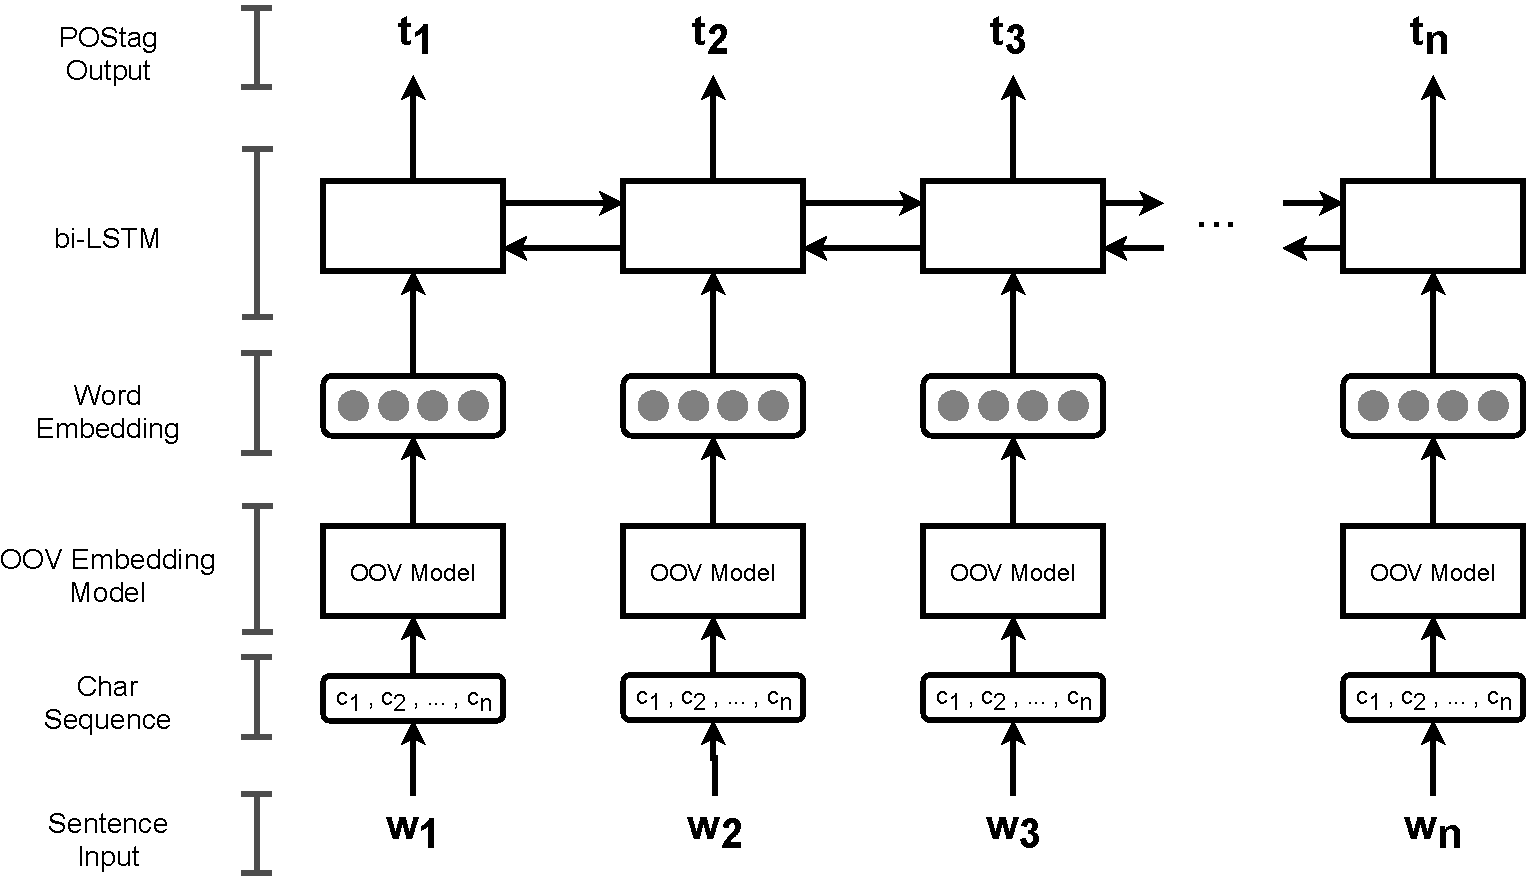
\includegraphics[width=.8\linewidth]{images/postag.pdf}
            \caption{Postagging Process}
            \label{fig:postag}
        \end{figure}
 
    \subsection{Word Similarity Tasks}
        Word similarity tasks is basically task to evaluate the
        similarities between two words based on human given scores.
        Generally, several human subject were given pairs of words and
        asked to score its similarities. Those scores then will be
        used to determine the agreements between subjects that certain
        word pairs have stronger connection and the others are weaker.
        In order to calculate the agreements between the OOV generated
        embedding and the data that is scored by human, Spearman's
        rank correlation coefficient is used. Firstly, given a pair
        $(w_1, w_2)$, the cosine distance of the embedding based on
        the generated OOV model between $e_1$ and $e_2$ for $w_1$ and
        $w_2$ respectfuly, are calculated using equation
        \ref{eq:cosinesim}. 

        \begin{equation}
            \label{eq:cosinesim}
            cosine\ similarity = \frac{e_1 \cdot e_2}{\Vert e_1 \Vert \Vert e_2 \Vert}
        \end{equation}

        After all of the cosine distance for all pairs are calculated,
        Spearman rank's correlation from the dataset and the generated
        embedding are calculated by using equation \ref{eq:spearman}
        and by using equation \ref{eq:spearmantied} when no tied ranks
        exists.
        
        \begin{align}
            \label{eq:spearman}
            \rho    &= \ddfrac{n\sum_{i=1}^n u_i v_i - \Bigg( \sum_{i=1}^n u_i \Bigg) \Bigg( \sum_{i=1}^n v_i \Bigg)}{\sqrt{\Bigg[ n \sum_{i=1}^n u_i^2 - \Bigg( \sum_{i=1}^n u_i \Bigg)^2 \Bigg] \Bigg[ n \sum_{i=1}^n v_i^2 - \Bigg( \sum_{i=1}^n v_i \Bigg)^2 \Bigg] }}\\
            \label{eq:spearmantied}            
                    &= 1 - \ddfrac{6 \sum_{i=1}^n d_i^2}{n(n^2 - 1)}\ \text{where}\ d_i = u_i - v_i
        \end{align}

\chapter{Implementation}
\label{chap:implementation}

\section{Datasets}
    \subsection{Pretrained Word Embedding}
        In order to train the model, pretrained embedding is needed
        since the model will tries to predict embedding of from known
        vocabulary $v \in \mathcal{V}$ with its known embedding $w \in
        \mathcal{W}$. For this purpose, word2vec which trained on
        Google news dataset using skip-gram model containing 3 million
        words and phrases \cite{Distributed2013mikolov}. Word2vec
        contains phrases from negative sampling and for the purpose of
        this research those phrases did not included. The embedding
        has 300 dimensional vectors. Only top 40 thousands words with
        removal if the word is actually a phrase.
        
        Another pretrained embedding is polyglot
        \cite{polyglot2013alrfou} which contains multilingual
        embeddings. For this research, only English embedding that
        contains around 100 thousands with 60 dimensional vector
        representation. This pretrained embedding is also used in OOV
        handling model \textsc{Mimick} \cite{mimicking2017Pinter}.
        This model is used as baseline model.

        Dict2vec is yet another word embedding that trained based on
        the definition of a word in dictionary
        \cite{dict2vect2017tissier}. Originally, this embedding was
        tested using word similarity tasks, hence this embedding is
        used as baseline model for word similarity tasks.

    \subsection{Word Similarity Dataset}
        Several word similarity dataset were used in order to increase
        the pair examples since for the datasets that is collected,
        the maximum number of pairs is 3000 pairs. Those datasets are
        asdf, sadf, asdf, asdf, asdf, asdf, sadg, and asdfsadf.

\section{Programming Language and Tools}
    The model was using PyTorch 1.0.1
    \cite{pytorch2017paszke} on top of Python 3.6. Most of the
    basic model, for instance 2d convolution layer, 2d maxpool
    layer, fully connected layer, bi-lstm, and many activation
    functions and loss function, thus will serve enough for the
    purpose of this research.
        
\section{Hardware}
    The model was trained on the freely available google colaboratory
    (links here) which gives randomized hardware specification, thus
    the exact hardware used cannot be determined. Nevertheless, this
    only affects the time needed to train the model not the results.

%-----------------------------------------------------
% Chapter: Conclusion
%-----------------------------------------------------
\chapter{Conclusion}
\label{chap:conc}

I was right all along.

\section{What was I right about?}

I was right about the following things.

\subsection{Previous theories were wrong}

People thought they understood, but they didn't.

\subsection{My new idea is right}

Of course.


%%%%%%%%%%%%%%%%%%%%%%%%%%%%
% BIBLIOGRAPHY
\clearpage
\phantomsection
\addcontentsline{toc}{chapter}{Bibliography}
\bibliography{bibli}
%%%%%%%%%%%%%%%%%%%%%%%%%%%%


%%%%%%%%%%%%%%%%%%%%%%%%%%%%
% START APPENDICES
\appendix
%%%%%%%%%%%%%%%%%%%%%%%%%%%%


%-----------------------------------------------------
% Appendix: Code
%-----------------------------------------------------
\chapter{Code}
\label{app:code}

\begin{verbatim}
10 PRINT "HELLO WORLD"
\end{verbatim}


%%%%%%%%%%%%%%%%%%%%%%%%%%%%
% END DOCUMENT
\end{document}
%%%%%%%%%%%%%%%%%%%%%%%%%%%%